\documentclass{article}

\usepackage[main=english,vietnamese]{babel}
\usepackage[T1]{fontenc}
\usepackage[utf8]{inputenc}
\usepackage[sexy]{evan}
\usepackage{matchsticks}
\usepackage{wrapfig}
\usepackage{listings}

\newtheorem{hint}{Hint}

\title{A picture is worth a thousand words - Part 1}
\author{Nghia Doan}
\date{\today}

\begin{document}

\maketitle

In this article, we will investigate a number of ways to \textit{prove area equality without writing lengthy proof.}
While it sounds simple, easy, and exciting, it is important that you need to improve your creating thinking in order to 
first understand the examples, and then use them as tools, guidelines, or ideas to solve the problems.

\begin{example*}[Example 1]
    $E$ is an arbitrary point inside the parallelogram $ABCD,$ prove that
    \[
        [AEB] + [CED] = \half [ABCD].
    \]
\end{example*}

\begin{figure}[h]
    \centering
    \begin{minipage}[t]{6.5cm}
        \begin{center}
            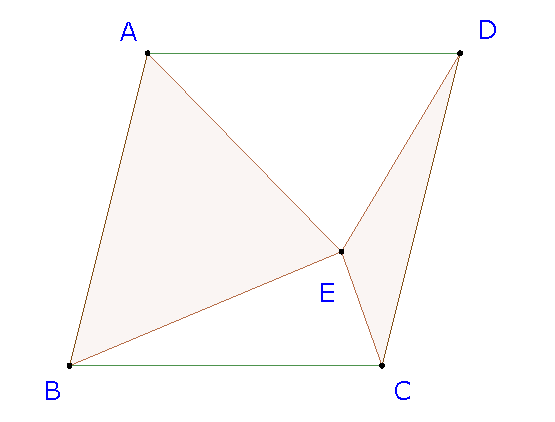
\includegraphics[width=5.5cm]{./svg/pdf/23-24-s3-i-p1.pdf}
        \end{center}
    \end{minipage}
    \qquad
    \begin{minipage}[t]{6.5cm}
        \centering
        \begin{center}
            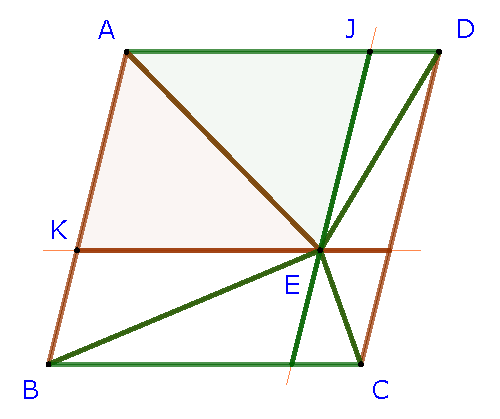
\includegraphics[width=5cm]{./svg/pdf/23-24-s3-i-p1-s.pdf}
        \end{center}
    \end{minipage}
\end{figure}

\begin{soln}
    Draw lines through $E,$ parallel with sides of $ABCD,$ dividing the parallelogram into four smaller parallelograms.
    Any of the smaller parallelogram, say $AKEJ$, consists of a brown triangle from the shaded triangle and a green triangles with the same area.
    Thus, the area of the shaded triangles is the sum of the area of all smaller brown triangles, which is half of the sum of the area of all smaller parallelograms,
    of half of the $ABCD$ parallelogram.
\end{soln}

\begin{remark*}
    Here's how we use the techniques:
    \begin{enumerate}[topsep=0pt, partopsep=0pt, itemsep=0pt]
        \ii First, divide the given figure into smaller figures.
        \ii Deal with each of them, iif they have the same shape, then work in the same way.
        \ii Use all partial results to arrive at the overall result.
    \end{enumerate}
\end{remark*}

\newpage

\begin{example*}[Example 2]
    $E$ and $F$ are midpoints of $BC$ and $DA$ in the convex quadrilateral $ABCD,$ prove that
    \[
        [AECF] = \half [ABCD].
    \]
\end{example*}

\begin{figure}[h]
    \centering
    \begin{minipage}[t]{6.5cm}
        \begin{center}
            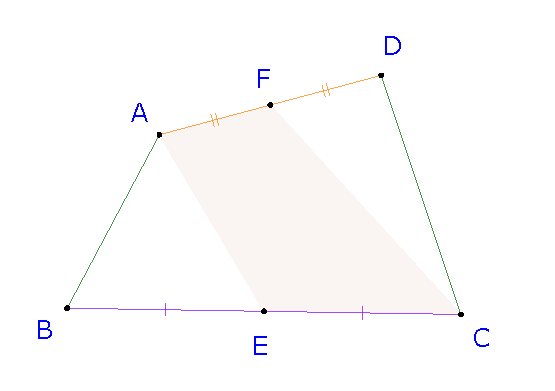
\includegraphics[width=6.5cm]{./svg/pdf/23-24-s3-i-p2.pdf}
        \end{center}
    \end{minipage}
    \qquad
    \begin{minipage}[t]{6.5cm}
        \centering
        \begin{center}
            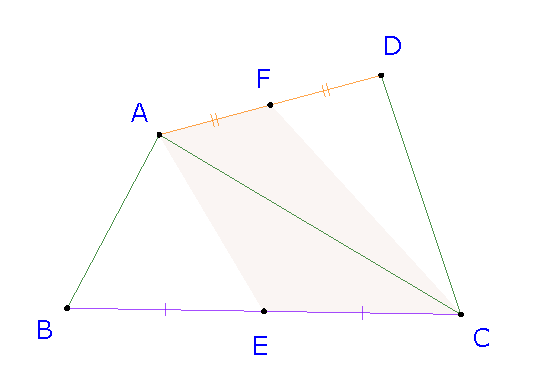
\includegraphics[width=6.5cm]{./svg/pdf/23-24-s3-i-p2-s.pdf}
        \end{center}
    \end{minipage}
\end{figure}

\begin{proof}
    Connect $AC.$ Since $E$ is midpoint of $BC,$ thus the triangles $ABE$ and $AEC$ have the same area.
    Similarly triangles $CDF$ and $CFA$ have the same area. Thus the area of $AECF$ is half of $ABCD.$
\end{proof}

\begin{example*}[Example 3]
    \label{example:23-24-s3-i-p3}
    $I$ is an arbitrary point on the diagonal $BD$ in parallelogram $ABCD.$
    Lines through $I$ parallel with the sides of $ABCD$ intersect $AB,$ $BC,$ $CD,$ and $DA$ at $E, F, G,$ and $H,$ respectively.
    \[
        [AEIH] = [FCGI].
    \]
\end{example*}

\begin{figure}[h]
    \centering
    \begin{minipage}[t]{6.5cm}
        \begin{center}
            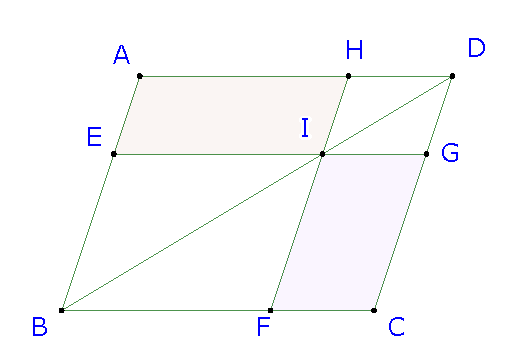
\includegraphics[width=6.5cm]{./svg/pdf/23-24-s3-i-p3.pdf}
        \end{center}
    \end{minipage}
    \qquad
    \begin{minipage}[t]{6.5cm}
        \centering
        \begin{center}
            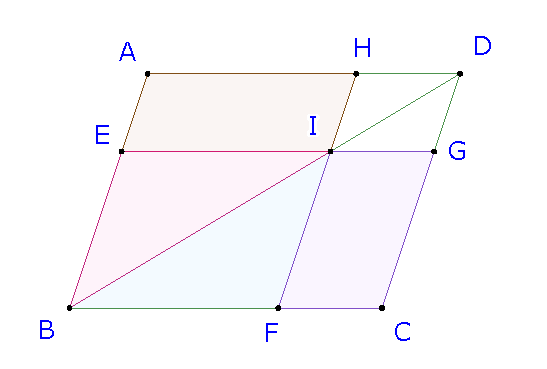
\includegraphics[width=6.5cm]{./svg/pdf/23-24-s3-i-p3-s.pdf}
        \end{center}
    \end{minipage}
\end{figure}

\begin{proof}
    First, since $BD$ is the diagonal in parallelogram $ABCD,$ $[ABD] = [BCD].$
    Now, $BEIF$ is also a parallelogram, thus $[BEI] = [BFI],$ similarly $[HID] = [IGD].$
    Therefore 
    \[
        [AEIH] = [ABD] - [BEI] - [HID] = [BCD] - [BFI] - [IGD] = [FCGI].
    \]
\end{proof}

\newpage

\begin{example*}[Example 4]
    \label{example:23-24-s3-i-p4}
    $G, H$ are midpoints of $BC, CD$ in th regular hexagon $ABCDEF.$
    $EG$ and $FH$ intersect at $I.$ Prove that
    \[
        [GCHI] = [EFI].
    \]
\end{example*}

\begin{center}
    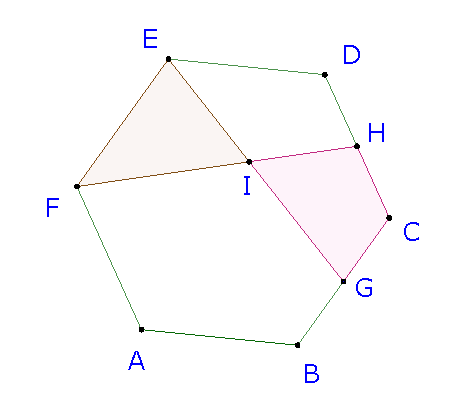
\includegraphics[width=6.5cm]{./svg/pdf/23-24-s3-i-p4.pdf}
\end{center}

\begin{proof}
    It is easy to see that the quadrilaterals $GCDE$ and $HDEF$ are congruent, thus have the same area, or $[GCDE] = [HDEF].$
    Taking $HDEI$ away, we have $[GCHI] = [EFI].$ 
\end{proof}

\begin{example*}[Example 5]
    $E, F, G,$ and $H$ are midpoints the sides in the convex quadrilateral $ABCD.$
    Prove that
    \[
        [EFGH] = \half [ABCD].
    \]
\end{example*}

\begin{center}
    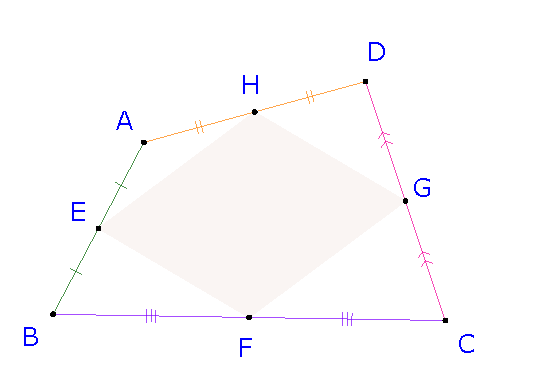
\includegraphics[width=6.5cm]{./svg/pdf/23-24-s3-i-p5.pdf}
\end{center}

\begin{proof}
    $EH$ is the mid-segment (the segment connecting two midpoints) in $\triangle ABD,$ therefore $[AEH] = \frac{1}{4}[ABD].$
    Similarly $[BEF] = \frac{1}{4}[ABC],$ $[CFG] = \frac{1}{4}[BCD],$ and $[GDH] = \frac{1}{4}[CDA],$ therefore:
    \[ 
        [AEH] + [BEF] + [CFG] + [GDH] = \half [ABCD] \Rightarrow [EFGH] = \half [ABCD].
    \]
\end{proof}

\end{document}